% \iffalse
%<*internal|cls|sty>
\def\Version{\the\year/\the\month/\the\day\ v0.0.1}
% \def\Version{2019/04/17 v0.0.1}
%</internal|cls|sty>
%<*internal>
\iffalse
%</internal>
%<cls|sty>\NeedsTeXFormat{LaTeX2e}[2005/12/01]
%<*cls&letter>
\ProvidesClass{HUBerlin-letter}
  [\Version\space Humboldt-Universität zu Berlin - letter documentclass]
\ClassInfo{HUBerlin}{* * * HUBerlin * * *\MessageBreak
    Part of the HUBerlin Bundle }
%</cls&letter>
%<*sty>
%<*style>
\ProvidesPackage{HUBerlin-bundle-style}
  [\Version\space HUBerlin - package for style the documentation]
  \PackageInfo{HUBerlin}{* * * HUBerlin * * *\MessageBreak
	  Part of the HUBerlin Bundle}
%</style>
%</sty>
%<*driver>
\catcode9=12
\ProvidesFile{\jobname.dtx}
	[\Version\space Documentation of the HUBerlin Bundle]
%</driver>
% /*
%       ██████  ███████  █████  ██████  ███    ███ ███████
% ▄ ██ ▄██   ██ ██      ██   ██ ██   ██ ████  ████ ██
%  ████ ██████  █████   ███████ ██   ██ ██ ████ ██ █████
% ▀ ██ ▀██   ██ ██      ██   ██ ██   ██ ██  ██  ██ ██
%       ██   ██ ███████ ██   ██ ██████  ██      ██ ███████
% */
%<*readme&main>
# HUBerlin
## Documents and Documentations for HUBerlin bundle

This bundle provides following files:

  * `HUBerlin-bundle.dtx` which is the core file designed with literate programming 
  * `HUBerlin-bundle.pdf` is documentation of the bundle.
  * `HUBerlin-letter.cls` is the documentclass for letters
  * `README.md`
  * `makefile`

Furthermore there are a couple of folders.
 * `examples`
 * `img`
 * `cls`


This work has the LPPL maintenance status _maintained_.
The current maintainer of this work is [Lukas C. Bossert](https://github.com/lukascbossert).
%</readme&main>
% /*
%     ██ ██████  ███████  █████  ██████  ███    ███ ███████
%    ██  ██   ██ ██      ██   ██ ██   ██ ████  ████ ██
%   ██   ██████  █████   ███████ ██   ██ ██ ████ ██ █████
%  ██    ██   ██ ██      ██   ██ ██   ██ ██  ██  ██ ██
% ██     ██   ██ ███████ ██   ██ ██████  ██      ██ ███████
% */
% /*
%       ██████  ██ ██████
% ▄ ██ ▄██   ██ ██ ██   ██
%  ████ ██████  ██ ██████
% ▀ ██ ▀██   ██ ██ ██   ██
%       ██████  ██ ██████
% */
%<*bib>
%%
%% Encoding: UTF-8
%%
@InCollection{Hoare1973,
  author = {Charles Antony Richard Hoare},
  title = {Hints on programming language design},
  editor = {C. Bunyan},
  booktitle = {Computer Systems Reliability},
  series = {State of the Art Report},
  number = {20},
  pages = {193--216},
  date = {1973},
  url={http://flint.cs.yale.edu/cs428/doc/HintsPL.pdf},
  urldate={2018-09-06},
  comment = {\blockcquote[195]{Hoare1973}{Documentation must be regarded as an integral part of the process of design and coding.
 A good programming language will encourage and assist the programmer to write clear,
 self-documenting code,
 and even perhaps to develop
 and display a pleasant style
 of writing.}}
}

%</bib>
% /*
%     ██ ██████  ██ ██████
%    ██  ██   ██ ██ ██   ██
%   ██   ██████  ██ ██████
%  ██    ██   ██ ██ ██   ██
% ██     ██████  ██ ██████
% */
%<*internal>
\fi
\def\nameofplainTeX{plain}
\ifx\fmtname\nameofplainTeX\else
  \expandafter\begingroup
\fi
%</internal>
% /*
%        ██ ███    ██ ███████
% ▄ ██ ▄██ ████   ██ ██
%  ████ ██ ██ ██  ██ ███████
% ▀ ██ ▀██ ██  ██ ██      ██
%        ██ ██   ████ ███████
% */
%<*install>
%% \CharacterTable
%%  {Upper-case    \A\B\C\D\E\F\G\H\I\J\K\L\M\N\O\P\Q\R\S\T\U\V\W\X\Y\Z
%%   Lower-case    \a\b\c\d\e\f\g\h\i\j\k\l\m\n\o\p\q\r\s\t\u\v\w\x\y\z
%%   Digits        \0\1\2\3\4\5\6\7\8\9
%%   Exclamation   \!     Double quote  \"     Hash (number) \#
%%   Dollar        \$     Percent       \%     Ampersand     \&
%%   Acute accent  \'     Left paren    \(     Right paren   \)
%%   Asterisk      \*     Plus          \+     Comma         \,
%%   Minus         \-     Point         \.     Solidus       \/
%%   Colon         \:     Semicolon     \;     Less than     \<
%%   Equals        \=     Greater than  \>     Question mark \?
%%   Commercial at \@     Left bracket  \[     Backslash     \\
%%   Right bracket \]     Circumflex    \^     Underscore    \_
%%   Grave accent  \`     Left brace    \{     Vertical bar  \|
%%   Right brace   \}     Tilde         \~}

\input docstrip.tex
\keepsilent
\askforoverwritefalse

\nopreamble\nopostamble

\usedir{doc/latex/\jobname}
\generate{
  \file{README.md}{\from{\jobname.dtx}{readme,main}}
  \file{HUBerlin-bundle-bibliography.bib}{\from{\jobname.dtx}{bib}}
  \file{examples/HUBerlin-letter.tex}{\from{\jobname.dtx}{example,letter}}
}

\preamble
----------------------------------------------------------------
HUBerlin-bundle
Author:  Lukas C. Bossert
E-mail:  lukas@texografie.de
License: Released under the LaTeX Project Public License v1.3c or later
See:     http://www.latex-project.org/lppl.txt
Various parts my have a different licence,
please consider and respect them carefully.
----------------------------------------------------------------

\endpreamble
\postamble
 
Copyright (C) 2019
\endpostamble

\usedir{tex/latex/\jobname}
\generate{
  \file{examples/HUBerlin-letter.tex}{\from{\jobname.dtx}{example,letter}}
  \file{examples/HUBerlin-letter.lco}{\from{\jobname.dtx}{example,lco}}
  \file{cls/HUBerlin-letter.cls}{\from{\jobname.dtx}{cls,letter}}
  %
  \file{HUBerlin-bundle-style.sty}{\from{\jobname.dtx}{sty,style}}
}
%</install>
%<install>\endbatchfile
%<*internal>
\usedir{source/latex/\jobname}
\generate{
  \file{\jobname.ins}{\from{\jobname.dtx}{install}}
}
\ifx\fmtname\nameofplainTeX
  \expandafter\endbatchfile
\else
  \expandafter\endgroup
\fi
%</internal>
% /*
%     ██ ██ ███    ██ ███████
%    ██  ██ ████   ██ ██
%   ██   ██ ██ ██  ██ ███████
%  ██    ██ ██  ██ ██      ██
% ██     ██ ██   ████ ███████
% */
%<*driver>
\ProvidesFile{\jobname.dtx}
	[\Version\space Documents and documentation for HUBerlin]
%</driver>
% /*
% ██████   ██████   ██████  ██████ ██       █████  ███████ ███████
% ██   ██ ██    ██ ██      ██      ██      ██   ██ ██      ██
% ██   ██ ██    ██ ██      ██      ██      ███████ ███████ ███████
% ██   ██ ██    ██ ██      ██      ██      ██   ██      ██      ██
% ██████   ██████   ██████  ██████ ███████ ██   ██ ███████ ███████
% */
%<*driver>
\def\HUBerlinsubject{Guideline}
\def\HUBerlinshort{HUBerlin-bundle}
\def\HUBerlintitle{%
Documents and Documentations for \LaTeX\ at the Humboldt-Universität zu Berlin}
\def\HUBerlinsubtitle{For Authors and Developers}
\def\HUBerlinauthor{Lukas C. Bossert}
\RequirePackage{scrlfile}
\PassOptionsToClass{%
	english
   ,oneside
  }{scrbook}
\ReplaceClass{article}{scrbook}
\documentclass{ltxdoc}
%\RecordChanges
% \EnableCrossrefs
% \CodelineIndex
\usepackage{HUBerlin-bundle-style} 
\GetFileInfo{\jobname.dtx}
% /*
%           ██████   ██████   ██████ ██    ██ ███    ███ ███████ ███    ██ ████████
% ▄ ██ ▄    ██   ██ ██    ██ ██      ██    ██ ████  ████ ██      ████   ██    ██
%  ████     ██   ██ ██    ██ ██      ██    ██ ██ ████ ██ █████   ██ ██  ██    ██
% ▀ ██ ▀    ██   ██ ██    ██ ██      ██    ██ ██  ██  ██ ██      ██  ██ ██    ██
%           ██████   ██████   ██████  ██████  ██      ██ ███████ ██   ████    ██
% */
\begin{document}
\openoutputfile{\jobname.pkglist}{pkglist}
\pdfbookmark[section]{\contentsname}{toc}
\tableofcontents
\clearpage
\chapter{Introduction}
\begin{markdown*}{hybrid=true}
%</driver>
% /*
%       ██████  ███████  █████  ██████  ███    ███ ███████
% ▄ ██ ▄██   ██ ██      ██   ██ ██   ██ ████  ████ ██
%  ████ ██████  █████   ███████ ██   ██ ██ ████ ██ █████
% ▀ ██ ▀██   ██ ██      ██   ██ ██   ██ ██  ██  ██ ██
%       ██   ██ ███████ ██   ██ ██████  ██      ██ ███████
% */
%<*driver|readme&main>
With this bundle you have several documents which are according to the coporate design of the Humboldt-Universität zu Berlin.

Following documents or documentclasses are available:

* letter (`HUBerlin-letter.cls`)



## Installation of the bundle
`HUBerlin` is part of the distributions [MiKTeX](http://www.miktex.org)
and [TeXLive](http://www.tug.org/texlive) -- thus, you
can easily install it using the respective package manager.
If you would like to
install `HUBerlin-bundle` into your local folder  manually, do the following:
Go to your terminal, browse to the folder of this bundle and run

```
make install
```


If you are using macOS you might be asked for your user account password for the installation.


Further options of this makefile are:

* `clean`:  deletes all unnecessary files
* `cleanbundle`:  deletes all files except `.dtx`, `.md`. You will get the plain version of this bundle.
This might be helpful if you send the bundle to someone else.
* `ctan`:  this will create a zip file which can be used to send to CTAN.
* `files`: will only create the files from the `.dtx`-scratch.
* `uninstall`: will erase the locally installed files.


This bundle is constantly updated. For hints, errors or suggestions use the GitHub repository [https://github.com/LukasCBossert/HUBerlin-bundle](https://github.com/LukasCBossert/HUBerlin-bundle).

## Changelog

All notable changes to this project will be documented in the [README.md](https://github.com/LukasCBossert/HUBerlin-bundle/blob/master/README.md).
This project **does not** adhere to [Semantic Versioning](http://semver.org/).
The markdown syntax is inspired by the conventions proposed by [keepachangelog.com](http://keepachangelog.com/).
%</driver|readme&main>
% /*
%     ██ ██████  ███████  █████  ██████  ███    ███ ███████
%    ██  ██   ██ ██      ██   ██ ██   ██ ████  ████ ██
%   ██   ██████  █████   ███████ ██   ██ ██ ████ ██ █████
%  ██    ██   ██ ██      ██   ██ ██   ██ ██  ██  ██ ██
% ██     ██   ██ ███████ ██   ██ ██████  ██      ██ ███████
% */
%<*driver>
\end{markdown*}
\chapter{Preambel}

This bundle consists of various files
which are either generated by the core file (|.dtx|)
or are part of the basic structure of this bundle.
You can easily pick up the basic file structure from \cref{HUBerlin:bundle-structure}.

\begin{figure}[!htb]
\footnotesize
\dirtree{%
.1 \HUBerlinFolder HUBerlin-bundle.
.2 HUBerlin-bundle.dtx\DTcomment{code and documentation}.
.2 \HUBerlinFolder examples\DTcomment{folder for examplary files}.
.3 HUBerlin-letter.tex \DTcomment{letter}.
.3 HUBerlin-letter.lco \DTcomment{datafile for letter}.
.3 HUBerlin-letter.pdf \DTcomment{letter}.
.2 \HUBerlinFolder img\DTcomment{folder for images}.
.3 texografie-logo.png\DTcomment{logo of \TeXografie}.
.2 makefile\DTcomment{makefile to generate all required files}.
.2 README.md\DTcomment{README file with information on installation}.
}
\caption{Structure of \texttt{HUBerlin} bundle}
\label{HUBerlin:bundle-structure}
\end{figure}

When you run the |makefile|
you get all these various files described above.


 

\DocInput{\jobname.dtx}

\printbibliography


\part{Example files}
\chapter{Letter}
\IfFileExists{examples/HUBerlin-letter.pdf}
  {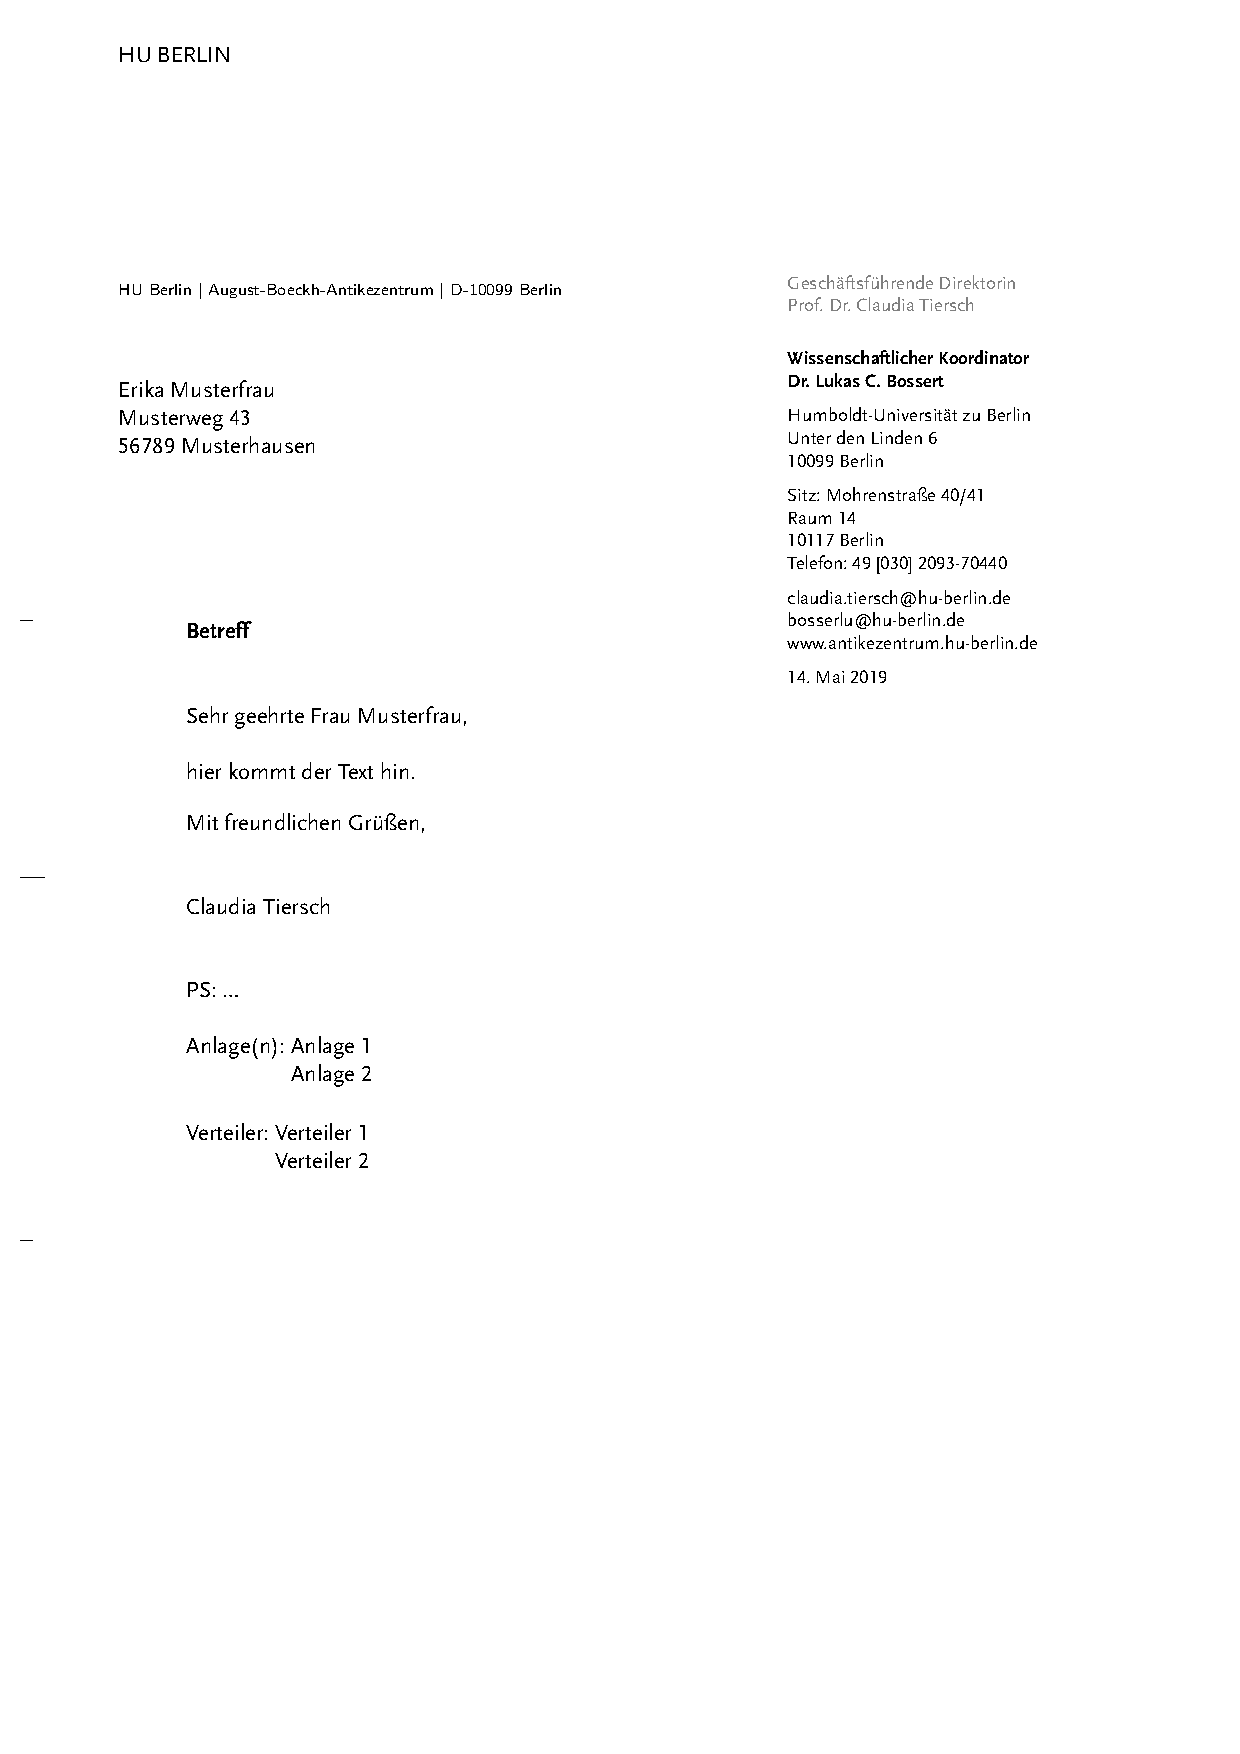
\includepdf[%
  pagecommand={\pagestyle{scrheadings}}
 ,link
 ,pages=-
 ,scale=.8
 % ,nup=1x2
 ,frame]{examples/HUBerlin-letter.pdf}}
 {|examples/HUBerlin-letter.pdf| missing!}

\end{document}
%</driver>
% /*
%     ██ ██████   ██████   ██████ ██    ██ ███    ███ ███████ ███    ██ ████████
%    ██  ██   ██ ██    ██ ██      ██    ██ ████  ████ ██      ████   ██    ██
%   ██   ██   ██ ██    ██ ██      ██    ██ ██ ████ ██ █████   ██ ██  ██    ██
%  ██    ██   ██ ██    ██ ██      ██    ██ ██  ██  ██ ██      ██  ██ ██    ██
% ██     ██████   ██████   ██████  ██████  ██      ██ ███████ ██   ████    ██
% */
% /*
%            ██████  ██████  ██████  ███████
%           ██      ██    ██ ██   ██ ██
% █████     ██      ██    ██ ██   ██ █████       █████
%           ██      ██    ██ ██   ██ ██
%            ██████  ██████  ██████  ███████
% */
% \fi
%
% \part{Guideline for Users} 
%    \begin{macrocode}
%<*example>
%    \end{macrocode}
% \chapter{Letter}
% We give an example on how to create a letter.
%
% \section{\texttt{.lco}-file}
%    \begin{macrocode}
%<*lco>
%    \end{macrocode}
%    \begin{macrocode}
\ProvidesFile{HUBerlin-letter.lco}

  

\setkomavar{fromname}{Dr. Lukas C. Bossert} % Name
\setkomavar{fromaddress}{%
  Humboldt-Universität zu Berlin\\
  Unter den Linden 6\\
  10099 Berlin}
\setkomavar{fromemail}{bosserlu@hu-berlin.de} % Email-Adresse
\setkomavar{fromphone}{49 [030] 2093-70440} % Telefonnummer
\setkomavar{fromurl}{www.antikezentrum.hu-berlin.de} % Website


\setkomavar{backaddress}{HU Berlin\\August-Boeckh-Antikezentrum\\D-10099 Berlin} 

\setkomavar{institute}{}%
\setkomavar{institute.head}[Prof. Dr.]{Claudia Tiersch}%
\setkomavar{institute.head.position}{Geschäftsführende Direktorin}%
\setkomavar{institute.head.mail}{claudia.tiersch@hu-berlin.de}%
\setkomavar{institute.logo}{%

\includegraphics[width=\useplength{locwidth}]{ABAZ-logo.png}
}%
\setkomavar{fromname.position}{Wissenschaftlicher Koordinator}
\setkomavar{local}{%
  %\def\\{\usekomavar{backaddressseparator}\@ogobble}
  Mohrenstraße 40/41\\
  Raum 14\\
  10117 Berlin}
\setkomavar{connections}{U2 Haltestelle Hausvogteiplatz}

% ===== Signatur =====
\setkomavar{signature}{%
  \usekomavar{institute.head}\\
}
\renewcommand*{\raggedsignature}{\raggedright}
%    \end{macrocode}
%    \begin{macrocode}
%</lco>
%    \end{macrocode}
% \section{\texttt{.tex}-file}
%    \begin{macrocode}
%<*letter>
%    \end{macrocode}
%    \begin{macrocode}
\documentclass{HUBerlin-letter}
%    \end{macrocode}
% Now we load the personal data-file which has the ending |.lco|.
%    \begin{macrocode}
\LoadLetterOption{HUBerlin-letter}
%    \end{macrocode}
% If you have the HU font installed on your computer, 
% you can load it:
%    \begin{macrocode}
\setmainfont[%
  BoldFont=ScalaSans-BoldLF,
  Numbers=OldStyle]{ScalaSans-RegularLF}
%    \end{macrocode}
%    \begin{macrocode}
\setkomavar{yourref}{}  % Ihr Zeichen
\setkomavar{yourmail}{}         % Ihr Schreiben vom
\setkomavar{myref}{}            % Unser Zeichen
\setkomavar{customer}{}         % Kundennummer
\setkomavar{invoice}{}          % Rechnungsnummer
\setkomavar{place}{Berlin} % Ort

\setkomavar{subject}{Betreff}
% =====================================
\begin{document}

\begin{letter}{%
% ===== Zielanschrift =====
  Erika Musterfrau\\
  Musterweg 43\\
  56789 Musterhausen%
% =======================
}



\opening{Sehr geehrte Frau Musterfrau,}

hier kommt der Text hin.

\closing{Mit freundlichen Grüßen,}

% ===== Postskriptum =====
\ps PS: \dots
% ========================

% ===== Anlage(n) =====
% \setkomavar*{enclseparator}{Anlage}
\encl{%
  Anlage 1\\
  Anlage 2%
}
% ===================

% ===== Verteiler =====
% \setkomavar*{ccseparator}{Kopie an}
\cc{%
  Verteiler 1\\
  Verteiler 2%
}
% =====================

\end{letter}
\end{document}
%    \end{macrocode}
% And how does a example letter looks like?
% \HUBerlinlisting%
%  [listing options = {%
%	,linerange={18-53}
%   ,numbers     = left
%   ,numbersep   = 10pt
%   ,numberstyle =\footnotesize\ttfamily\color{HUBerlin-grey}
%   }]%
%  {examples/HUBerlin-letter.tex}
%    \begin{macrocode}
%</letter>
%</example>
%    \end{macrocode}
%
%\part{Guide for Coders}
%    \begin{macrocode}
%<*cls>
%    \end{macrocode}
%\chapter{Letter}
%    \begin{macrocode}
%<*letter>
%    \end{macrocode}
%    \begin{macrocode}
\RequirePackage{xkeyval}
%    \end{macrocode}
%    \begin{macrocode}
\DeclareOptionX*{\OptionNotUsed}
\ProcessOptionsX\relax
\LoadClass[%
  fontsize=11pt,
  version=last,
  DIN,
]{scrlttr2}
%    \end{macrocode}
%    \begin{macrocode}
\RequirePackage{ifluatex,luatex85}
\ifluatex
\else
\GenericError{HUBerlin}%
 {Please use `LuaLaTeX' as Compiler.^^J I abort here.}
\fi
%    \end{macrocode}
%
%    \begin{macrocode}
\RequirePackage[ngerman]{babel}
\RequirePackage{graphicx}
\RequirePackage{xcolor}
\RequirePackage{fontspec}
%    \end{macrocode}
%
%    \begin{macrocode}
% HU DESIGN %
\setkomavar{backaddressseparator}{~\textbar~}
\KOMAoptions{%
locfield=wide,          % Breite Absenderergänzung (location)
fromalign=left,         % Ausrichtung des Briefkopfes
numericaldate=false,
refline=nodate,
backaddress=plain,
}


\setkomavar{location}{%
  \raggedright
  \footnotesize{%
  \begingroup
  \color{black!50}
   \ifkomavarempty{institute.logo}
    {\usekomavar{institute}}
    {\usekomavar{institute.logo}}\\%
  \usekomavar{institute.head.position}\\%
  \usekomavar*{institute.head}\space\usekomavar{institute.head}\\%
  \endgroup
  \vspace*{.5cm}
  {\bfseries%
  \usekomavar{fromname.position}\\
  \usekomavar{fromname}}\\
  \vspace*{.5\baselineskip}
  \usekomavar{fromaddress}
  \vspace*{.5\baselineskip}\\
  \usekomavar*{local}\space\usekomavar{local}\\
  \usekomavar*{fromphone}\usekomavar{fromphone}
  \ifkomavarempty{fromfax}{}{\usekomavar*{fromfax}\usekomavar{fromfax}}
  \vspace*{.5\baselineskip}\\
  \ifkomavarempty{institute.head.mail}{}{\usekomavar{institute.head.mail}}
  \usekomavar{fromemail}
  \usekomavar{fromurl}\\
  \vspace*{.5\baselineskip}
  \usekomavar{date}}%
}
% ============================
\setkomavar{firsthead}{%
  \parbox{\linewidth}{%
 
\includegraphics[width=.8\linewidth]{HUBerlin-logo.png}
  }%
}

 % \@setplength{locheight}{length } 
 % \@setplength{lochpos}{length } 
 % \@setplength{locvpos}{length } 
 % \@setplength{locwidth}{length }

\setkomavar{title}{}
\setkomavar{date}{\today}
%    \end{macrocode}
% We define new |komavar|s.
%    \begin{macrocode}
\newkomavar{institute}%
\newkomavar{institute.head}%
\newkomavar{institute.head.position}%
\newkomavar{institute.head.mail}%
\newkomavar{institute.logo}%
\newkomavar{fromname.position}
\newkomavar[Sitz:]{local}
\newkomavar[Verkehrsverbindungen]{connections}
%    \end{macrocode}
%    \begin{macrocode}
%</letter>
%    \end{macrocode}
%    \begin{macrocode}
%</cls>
%    \end{macrocode}
%\chapter{Documentation preamble \param{style}}
%    \begin{macrocode}
%<*sty>
%<*style>
\makeatletter
\addtolength\marginparwidth{-40pt}
\addtolength\marginparsep{4mm} 
\addtolength\oddsidemargin{-20pt}
\addtolength\evensidemargin{-20pt}
\let\PrintDescribeMacro=\@gobble
\let\PrintDescribeEnv=\@gobble
% \def\Describe@Macro#1{\endgroup
%     %\marginnote{\PrintDescribeMacro{#1}}%
%     \SpecialUsageIndex{#1}\@esphack\ignorespaces%
%     }
%\def\Describe@Env#1{\endgroup
%     %\marginnote{\PrintDescribeEnv{#1}}%
%     \SpecialEnvIndex{#1}\@esphack\ignorespaces%
%     }
\makeatother
\AtBeginDocument{\normalmarginpar}
\setlength\MacrocodeTopsep{\baselineskip}
\setlength\MacroIndent{6mm}


\RequirePackage{luatexbase}
\RequirePackage[ngerman,english]{babel}
\RequirePackage{calc} 

\RequirePackage[
  paper      = a4paper,  %  - use A4 paper size
  foot       = 2cm,
  inner      = 3cm,  %  - total body: left margin (odd pages)
  top        = 3cm,  %  - total body: top margin
  outer      = 3cm,  %  - total body: right margin (odd pages)
  bottom     = 3cm,  %  - total body: bottom margin
  marginparwidth = 2cm,  %  - width for side note
  marginparsep   = .5cm,  %  - space between notes and body text (content)
%  showframe,
]{geometry}

\newlength\fullwidth
\setlength\fullwidth{\textwidth+\marginparwidth+\marginparsep}

\KOMAoptions{
	numbers    = noenddot,
}
\AtBeginDocument{
  \KOMAoptions{
	% headwidth  = {\fullwidth},
	% footwidth  = {\fullwidth},
	footheight = 20pt,
	headheight = 29pt,
	captions   = tableheading,
}}



\title{\HUBerlintitle}
%\subtitle{\HUBerlinsubtitle}
\author{\HUBerlinauthor}
\date{\Version}


%---- Required Packages
\RequirePackage{ifluatex,luatex85}


\ifluatex% LuaTeX
\else
\GenericError{HUBerlin}{Please use `LuaLaTeX' as Compiler.^^J I abort here.}
\fi
%    \end{macrocode}
% For fonts we load the package \pkg{fontspec} which
% has almost no limits handling font-stuff.
%    \begin{macrocode}
\RequirePackage{fontspec}
%    \end{macrocode}
%    \begin{macrocode}
\RequirePackage[mono=false]{libertine}
\RequirePackage{amssymb}

\defaultfontfeatures{%
  Ligatures = TeX
 ,Scale     = MatchLowercase
 ,Numbers   = OldStyle
}
%    \end{macrocode}
% For fonts we use the available |TeX Gyre Pagella| as main font.\fnurl{http://www.gust.org.pl/projects/e-foundry/tex-gyre}
%    \begin{macrocode}
\setmainfont[%
   Ligatures = TeX
  ,Numbers   = OldStyle]{TeX Gyre Pagella}
%    \end{macrocode}
% And we declare also the other fonts, too.
%    \begin{macrocode}
\setmonofont[Scale=1]{TeX Gyre Cursor}
\setsansfont[%
  ,LetterSpace = .8]{TeX Gyre Adventor-Regular}
\linespread{1.05}
%    \end{macrocode}
%    \begin{macrocode}
\newfontfamily\listingsfont[ 
  Scale     = MatchLowercase,
]{TeX Gyre Cursor}
\renewcommand\MacroFont{\listingsfont}

\RequirePackage{marginnote}
\renewcommand*{\marginfont}{%
  \rule{0pt}{0.7\baselineskip}%
  \footnotesize%
  \color{HUBerlin-brown}}

\RequirePackage[
  german = guillemets,
  style  = german,
]{csquotes}

\RequirePackage{enumitem}
\setlist{
  nosep, 
  % itemindent=1em,
  % labelindent=0.5\parindent,
  leftmargin=*}
\newlist{tabitemize}{itemize}{2}% neue Listenumgebung 
\setlist[tabitemize]{%
  nosep, 
  leftmargin=*
 } 
\setlist[tabitemize,1]{label=\labelitemi} 
\setlist[tabitemize,2]{label=\labelitemii} 


\clubpenalty=10000  % prevent single lines at the beginning of a paragraph (Schusterjungen)
\widowpenalty=10000  % prevent single lines at the end of a paragraph (Hurenkinder)
\displaywidowpenalty=10000    %

\RequirePackage{pdfpages}
\RequirePackage{biblatex}
\addbibresource{\jobname-bibliography.bib}
\addbibresource{\jobname-ctan.bib}
\RequirePackage{ccicons} %creative commons
\RequirePackage{xparse}
\RequirePackage{ragged2e}
\RequirePackage{microtype}
\RequirePackage{xspace}
\RequirePackage{graphicx}
\graphicspath{{img/}}
%    \end{macrocode}
% The \pkg{luaimageembed} is to embed the image based out of code.
%    \begin{macrocode}
\RequirePackage{luaimageembed}
%    \end{macrocode}
%    \begin{macrocode}
\RequirePackage{etoolbox}
%https://tex.stackexchange.com/a/235881/98739
\AfterEndPreamble{\maketitle}

% https://tex.stackexchange.com/a/401466/98739
\makeatletter
\renewcommand*{\maketitle}{%
  % taken and shortened from /usr/share/texmf/tex/latex/koma-script/scrartcl.cls
  \begin{titlepage}
  \newgeometry{left=3cm,right=3cm,top=1.5cm,bottom=2cm}
  \global\@topnum=\z@
  \setparsizes{\z@}{\z@}{\z@\@plus 1fil}\par@updaterelative
  \null
   {\large\@author\hfill Guideline and Documentation\par}
  \vskip 10em%
	{\begin{center}\color{HUBerlin-blue}
	{\fontsize{50}{55}\selectfont\HUBerlinshort{} \par\vskip .5em%
	\Large\sffamily\@title}\par
	\vskip .5em
	\end{center}}%
	{\ifx\@subtitle\@empty\else\usekomafont{subtitle}\@subtitle\par\fi}%
	\null\vskip 5em%
	\blockcquote[195]{Hoare1973}{Documentation must be regarded as an integral part of the process of design and coding.
 A good programming language will encourage and assist the programmer to write clear,
 self-documenting code,
 and even perhaps to develop
 and display a pleasant style
 of writing.}
	\null\vfill
	{\usekomafont{subtitle}{\@date \hfill
	
\includegraphics[width=4cm]{texografie}\\}}%
  \par
 \vskip 0em
  \restoregeometry
  \end{titlepage}
}%
\makeatother

\RequirePackage{xcolor}
\definecolor{HUBerlin-blue}{RGB}{0,65,137} % HEX 004189
\definecolor{HUBerlin-green}{RGB}{150,190,20} % HEX 93C11A % Topoi
\definecolor{HUBerlin-grey}{RGB}{169,169,169}
\definecolor{HUBerlin-brown}{RGB}{82,79,60}
\definecolor{HUBerlin-red}{RGB}{180,0,0}


\usepackage{dirtree}
\renewcommand*\DTstylecomment{%
  \color{HUBerlin-grey}%
  \footnotesize%
  \sffamily}
\renewcommand*\DTstyle{%
  \ttfamily%
  \small%
  }

\RequirePackage[ 
  markcase    = noupper,
  footsepline = .5pt,
  % headsepline = .5pt,
  autooneside = false,% use left and right marks with a onesided document
  automark,% set \leftmark and \rightmark automatically by *\section and \subsection
  draft  = false,
  ]{scrlayer-scrpage} 

\pagestyle{scrheadings}
\clearscrheadfoot
\rofoot*{\thepage}
\lofoot*{\textcolor{HUBerlin-blue}{\HUBerlintitle}\ \vrule\ \textcolor{HUBerlin-brown}{\HUBerlinsubtitle}}
\rohead*{HUBerlin-bundle}
\lohead*{Version: \Version}
%    \end{macrocode}
%    \begin{macrocode}
% https://tex.stackexchange.com/a/352925/98739
\newcommand*\partnumber{}
\DeclareNewLayer[
  background,
  textarea,
  addwidth=\marginparsep+\marginparwidth,
  mode=picture,
  contents={%
	\putC{\makebox[0pt][c]{\raisebox{-.5\height}{\scalebox{50}{\textcolor{black!5}{\partnumber}}}}}\gdef\partnumber{}%
  }
]{partnumber}
\DeclareNewPageStyleByLayers{part}{partnumber}
\renewcommand\partpagestyle{part}
\renewcommand*{\partformat}{\gdef\partnumber{\thepart}}

% only a dirty workaround for the part title
\newcommand*\changedpartwidth[1]{%
  \makebox[\linewidth][l]{%
	\parbox{\dimexpr\textwidth+\marginparsep+\marginparwidth\relax}{\raggedpart#1}%
  }%
}
% add \changedpartwidth as last command to the settings for font element part
\addtokomafont{part}{\Huge\changedpartwidth}



%-https://tex.stackexchange.com/a/339516/98739 | https://tex.stackexchange.com/a/96722/98739
% footnotes in the footer:
\deffootnote%
  %[\normalparindent]%<width of mark>
  {0.0cm}%<indent of footnote text>
  {\normalparindent}%<paragraph indent in the footnote text>
  {\makebox[\normalparindent][r]%
  {\thefootnotemark\hspace*{3pt}}}%<definition of mark>
\newlength{\normalparindent}
\AtBeginDocument{\setlength{\normalparindent}{\parindent}}
 \setfootnoterule{0pt}% Kein Fußnotenstrich
 %\setfootnoterule[<height>]{<length>}

%    \end{macrocode}
% This will put the numbers of the chapters and sections into the margin.
%    \begin{macrocode}
\renewcommand\sectionlinesformat[4]{%
  \makebox[0pt][r]{#3}#4%
}
%    \end{macrocode}
%    \begin{macrocode}
\RequirePackage{url}
%  \urlstyle{same}

\setkomafont{title}{\sffamily\color{HUBerlin-blue}\flushleft\bfseries}
\setkomafont{disposition}{\color{HUBerlin-brown}\sffamily\bfseries\large}
\setkomafont{section}{\usekomafont{disposition}}
\setkomafont{subsection}{\usekomafont{disposition}}
\setkomafont{subsubsection}{\usekomafont{disposition}}
% \setkomafont{paragraph}{\bfseries}
% \setkomafont{subsubsection}{\sffamilybold}
\setkomafont{subtitle}{\large\color{HUBerlin-brown}\sffamily\flushleft}
\setkomafont{pageheadfoot}{\footnotesize\sffamily\color{HUBerlin-grey}}
\setkomafont{descriptionlabel}{\bfseries}
\setkomafont{footnotelabel}{\bfseries}
\addtokomafont{titlehead}{\flushright}
% \setkomafont{headsepline}{\color{HUBerlin-blue}}
%\setkomafont{marginnote}{\MakeUppercase\color{HUBerlin-brown}} 
\addtokomafont{caption}{\scriptsize}
\setkomafont{captionlabel}{\bfseries\sffamily}
\setkomafont{subject}{\bfseries\sffamily}
\setcapindent{0pt}

\raggedbottom

\usepackage{listings}
\PassOptionsToPackage{final}{listings}
\usepackage[%
   skins
  ,listings
  ,breakable
  ,xparse
  ,documentation
]{tcolorbox}
\lstMakeShortInline[language=TeX,basicstyle=\ttfamily]|
%    \end{macrocode}
% Following we load \pkg{hyperxmp} and \pkg{hyperref} for \pdf-meta data and interactive linked text.
%    \begin{macrocode}
\RequirePackage{hyperxmp}
\RequirePackage{hyperref}
\hypersetup{% setup the hyperref-package options
  unicode    = true,
  pdfauthor      = {HUBerlin}, %   - author (PDF meta)
  pdfauthortitle     = {},
  pdfcopyright   = {Copyright (c) \the\year . All rights reserved.},
  pdfhighlight   = /N,
  pdfdisplaydoctitle = true,
  pdfdate    = {\today},
  pdflang    = {},%de en
  pdfcaptionwriter   = {Lukas C. Bossert},
  pdfkeywords    = {HUBerlin},
  pdfencoding    = auto,
  pdfproducer    = {HUBerlin with LuaLaTeX},
  bookmarksnumbered  = true,    
  bookmarksopenlevel = 2,
  bookmarksopen  = true,    
  bookmarksdepth = 3,
  colorlinks     = true,    %Colours links instead of ugly boxes
  urlcolor       = HUBerlin-blue,    %Colour for external hyperlinks
  linkcolor      = black,   %Colour of internal links
  citecolor      = black,   %Colour of citations
  linktoc        = page,
  pdfborder      = {0 0 0},
  breaklinks     = true,  %allow line break inside links
}
\RequirePackage{bookmark}

\RequirePackage[
  sort,
  nameinlink,
  compress,
  ngerman,english
]{cleveref}


%---- newcommands
\newcommand{\TeXografie}{Lukas C. Bossert
  (www.TeXografie.de)}
\newcommand\HUBerlin{\HUBerlintitle\xspace}


\newcommand\HUBerlinFolder{%
  \begingroup%
  \normalfont%
  \color{HUBerlin-blue}%
  % \faFolderOpen% taken from fontawesome
  \hspace{.3em}%
  \endgroup}



\RedeclareSectionCommands[
  tocraggedpagenumber,
  toclinefill=\tocpageseparator,
  tocindent=0em,
  tocnumwidth=4em,
  tocpagenumberbox=\tocpagenumberbox% <- added
%  tocpagenumberformat=\textsf,
]{chapter,section,subsection,subsubsection,paragraph}

\newcommand\tocgobble[1]{}% <- added
\newcommand\tocpageseparator{\footnotesize\,\mbox{---}\,}
\newcommand\tocpagenumberbox[1]{\mbox{#1}}% <- added
\KOMAoptions{toc=indentunnumbered}

\RedeclareSectionCommand[
%  tocbeforeskip=1.25em plus 1pt
   ,tocentryformat=\large\scshape%
   ,tocindent=0em
   ,tocnumwidth=4em
   ,tocpagenumberbox=\tocgobble% <- added
]{part}
%\addtokomafont{partentry}{\scshape\sffamily\bfseries}
 
\RedeclareSectionCommand[%
%    ,beforeskip=1.15em plus 1pt%
	,tocentryformat=\textbf%
  %  ,toclinefill={\TOCLineLeaderFill}%\TOCLineLeaderFill[\textbf{.}]
]{chapter}




\newtcolorbox{example}[1][]{
  breakable,
  top=5pt,
  bottom=5pt,
  colback=HUBerlin-blue!10,
  colframe=HUBerlin-blue,
  left=5pt,
  right=5pt,
   sharp corners,
  boxrule=0pt,
  bottomrule=2pt,
  toprule=2pt,
   enhanced jigsaw,
  lefttitle=0pt,
   coltitle=white,
   fonttitle=\bfseries,
   fontupper=\small,%\ttfamily,
  % colbacktitle=HUBerlin-blue!20
  #1,
}

% Replace the squat-u symbol for spaces
% https://tex.stackexchange.com/a/488123/98739
\makeatletter
\def\lst@visiblespace{\lst@ttfamily{\char32}$\textcolor{HUBerlin-grey}{\cdot}$}
\makeatother


\lstset{%
  basicstyle = \linespread{0.7}\listingsfont
 ,breaklines = true
 ,breakatwhitespace
 ,alsoletter=\\\{\}\*\[\]\-
 ,showstringspaces=true
 }

\lstdefinestyle{HUBerlinlistingstyledef}{%
  tabsize      = 4,
  breaklines   = true,
  breakatwhitespace = true,
  postbreak=\mbox{$\hookrightarrow$},
  %keepspaces   = true,
  escapeinside = {(*@}{@*)},
  moredelim    = {[is][\ttfamily\bfseries\color{HUBerlin-blue}]{|}{|}},
  moredelim    = {[is][\ttfamily\bfseries\color{HUBerlin-blue}]{|1}{1|}},
  moredelim    = {[is][\ttfamily\bfseries\color{HUBerlin-red}]{|2}{2|}},
  aboveskip=0pt,
  belowskip=0pt,
  captionpos=b,
  resetmargins=true, 
  sensitive=true,
  upquote=true,
  showspaces=true,
  showtabs=true,
  tab=\textcolor{HUBerlin-grey}{\rightarrowfill},
  %numbers=left,
  %numberstyle=\footnotesize\ttfamily\color{HUBerlin-grey},
  comment      = [l]{\%},
  commentstyle = \footnotesize\color{HUBerlin-grey}\addfontfeature{LetterSpace=.7},
  % deletecomment = [l]{\%<}
  % morecomment  = [l][\nullfont]{\%<},
  % deletecomment  = [is]{\%<}{>},
}

\lstdefinestyle{HUBerlinlistingstyle}{%
  language  = {TeX},
  style     = {HUBerlinlistingstyledef},
}






\tcbset{%
HUBerlinstyle/.style={%
  enhanced,
  before skip=2mm,
  after skip=3mm,
  boxrule=0.7pt,
  left=2mm,
  right=2mm,
  top=2mm,
  bottom=2mm,
  sharp corners,
  colback=white,
  colbacklower=white,
  % fonttitle=\sffamily\bfseries,
  breakable,
  %before skip=\baselineskip,
  coltitle=white,
  colbacktitle=HUBerlin-blue!50!black,
  fonttitle=\bfseries\sffamily\footnotesize,
  % before upper={\mynote{\thetcbcounter}},
  title={\hfill{Example \thetcbcounter}},
  },
codecomment/.style={%
  listing outside comment,%
  boxrule=0pt,
  colback=white,
  }
}

\newtcolorbox{warning}[1][]{
  enhanced,
  before skip=2mm,
  after skip=3mm,
  boxrule=0.7pt,
  left=5mm,
  right=2mm,
  top=2mm,
  bottom=2mm,
  colback=white,
  colframe=yellow!20!black,
  sharp corners,
  rounded corners=southeast,
  arc is angular,
  arc=3mm,
  underlay={%
	\path[fill=HUBerlin-grey!80!black] ([yshift=3mm]interior.south east)--++(-0.4,-0.1)--++(0.1,-0.2);
	\path[draw=HUBerlin-grey,shorten <=-0.05mm,shorten >=-0.05mm] ([yshift=3mm]interior.south east)--++(-0.4,-0.1)--++(0.1,-0.2);
	\path[fill=red!50!black,draw=none] (interior.south west) rectangle node[white]{\Huge\bfseries !} ([xshift=4mm]interior.north west);
	},
  drop fuzzy shadow,
  #1
  }

\newtcblisting[%
  auto counter,
  crefname   = {example}{examples},
  Crefname   = {Example}{Examples},
]{codetext}[2][]{%
  HUBerlinstyle,
%  side text,
  rounded corners=northeast,
  arc=6mm,
  listing style=HUBerlinlistingstyle,
  label = #2,
  #1,
  }

\newtcblisting[%
  use counter from=codetext,
  crefname={code example}{code examples},
  Crefname={Code example}{Code examples}%
]{code}[2][]{%
  HUBerlinstyle,
  rounded corners=southeast,
  arc=6mm,
  listing only,
  listing style=HUBerlinlistingstyle,
  label = #2,
  #1,
}


\DeclareTCBInputListing[%
  use counter from=codetext,
  crefname={code example}{code examples},
  Crefname={Code example}{Code examples}%
]{\HUBerlinlisting}{ O{} m }{%
  HUBerlinstyle,
  listing file={#2},
  listing only,
    listing style=HUBerlinlistingstyle,
  #1,
}

%    \end{macrocode}
%    \begin{macrocode}
\makeatletter
\newrobustcmd*{\fnurl}[1][]{\hyper@normalise\ltd@fnurl{#1}}
\def\ltd@fnurl#1#2{\footnote{#1\hyper@linkurl{\Hurl{#2}}{#2}}}
\makeatother
%    \end{macrocode}
% The first command is used to refrence packages with:
% \cmd{\pkg}\marg{package name}.\footnote{Do not forget to
% insert the name of the package into the makefile
% in the definition of |PKG|.}
% The name of the package is linked to its entry on CTAN and
% refrenced to the bibliography in the end of this documentation.
%    \begin{macrocode}
\RequirePackage{newfile}
\newoutputstream{pkglist}
%    \end{macrocode}
%    \begin{macrocode}
\NewDocumentCommand{\pkg}{om}{%
  \IfNoValueTF{#1}
	{\lowercase{\href{http://www.ctan.org/pkg/#2}}{\textbf{#2}}}
	{\lowercase{\href{http://www.ctan.org/pkg/#1-#2}}{\textbf{#2}}}%
	\space\cite{#2}%
	\addtostream{pkglist}{#2}}
%    \end{macrocode}
%    \begin{macrocode}
\newrobustcmd*{\lit}[1]{\textsf{#1}}
\newrobustcmd*{\Code}[1]{\texttt{#1}}
\newrobustcmd*{\tex}{\TeX}
\newrobustcmd*{\etex}{\mbox{e-TeX}}
\newrobustcmd*{\pdftex}{pdf\-\tex}
\newrobustcmd*{\xetex}{Xe\-\tex}
\newrobustcmd*{\luatex}{Lua\-\tex}
\newrobustcmd*{\latex}{\LaTeX}%{La\kern-0.07em TeX}
\newrobustcmd*{\pdflatex}{pdf\-\latex}
\newrobustcmd*{\xelatex}{Xe\-\latex}
\newrobustcmd*{\lualatex}{Lua\-\latex}
\newrobustcmd*{\miktex}{Mik\-\tex}
\newrobustcmd*{\texlive}{\tex~live}
\newrobustcmd*{\bibtex}{Bib\kern-0.07em TeX}
\newrobustcmd*{\lppl}{\latex{} Project Public License}
\newrobustcmd*{\pdf}{{PDF}}
\newrobustcmd*{\md}{{MarkDown}}
\newrobustcmd*{\utf}{\mbox{{UTF}-8}}
% no \mbox here, we may have to break things
\newrobustcmd*{\bibfield}[1]{\Code{#1}}
\newrobustcmd*{\opt}[1]{\Code{#1}}
\newrobustcmd*{\bibmacro}[1]{\Code{#1}}
\newrobustcmd*{\bibtype}[1]{\Code{@#1}}
%\renewrobustcmd*{\cmd}[1]{\Code{\textbackslash #1}}
\renewrobustcmd\meta[1]{\normalfont{\textlangle}{\itshape#1\/}{\textrangle}}

% directly taken from ltxdoc.dtx
\renewrobustcmd\marg[1]{%
  {\ttfamily\textcolor{HUBerlin-red}{\{}}%
   \meta{#1}%
  {\ttfamily\textcolor{HUBerlin-red}{\}}}%
  }

\renewrobustcmd\oarg[1]{%
  {\ttfamily\textcolor{HUBerlin-green}{[}}%
   \meta{#1}%
  {\ttfamily\textcolor{HUBerlin-green}{]}}%
  }

% adapted from listings.dtx (lstdoc.sty)
\renewrobustcmd\cmd[1]{%
  \texttt{\color{HUBerlin-blue}\textbackslash\string#1}\xspace%
  }

\newrobustcmd\env[2][]{%
  \texttt{%
	\color{HUBerlin-blue}%
	\textbackslash begin\{\string#2\}#1}%
  \ldots
  \texttt{%
	\color{HUBerlin-blue}%
	\textbackslash end\{\string#2\}}%
  \xspace}
%    \end{macrocode}
% For a common layout of the parameter style to identify code
% of the different documents, files and packages we use
% \cmd{\param}\marg{name of the parameter}.
%    \begin{macrocode}
\newcommand\param[1]{%
  \begingroup%
  \normalfont%
  \ttfamily%
  \bfseries%
  \textless%
  #1%
  \ttfamily%
  \bfseries%
  \textgreater%
  \endgroup}
%    \end{macrocode}
%    \begin{macrocode} 
\pdfstringdefDisableCommands{%
 \def\lstinline#1{<#1>}
 \def\tex{TeX}%
 \def\etex{e-TeX}%
 \def\xetex{XeTeX}%
 \def\latex{LaTeX}%
 \def\xelatex{XeLaTeX}%
 \def\bibtex{BibTeX}%
 \def\lppl{LaTeX Project Public License}%
 \def\pdf{PDF}%
 \def\utf{UTF-8}%
 \def\\{}%
 \def\texttt#1{<#1>}%
 \def\marg#1{\{#1\}}%
 \def\oarg#1{[#1]}%
 \def\color#1#2{}%
 \def\env#1{<#1>}
 \def\cmd#1{#1}
}
% https://tex.stackexchange.com/a/24067/98739
\makeatletter
\patchcmd{\scr@startchapter}{\if@openright\cleardoublepage\else\clearpage\fi}{}{}{}
\makeatother
%
\usepackage[tightLists=false]{markdown}
\markdownSetup{rendererPrototypes={%
	link = {\href{#3}{#1}}%
}}
%</style>
%    \end{macrocode}
%    \begin{macrocode}
%</sty>
%    \end{macrocode}